\documentclass{beamer}
\usepackage[latin1]{inputenc}
\usepackage{graphicx}
\usetheme{Pittsburgh}
\title[Role of IT in the Classroom]{The Role of Computers, IT\\and the Internet in the Classroom}
\author{Josh Wainwright}
\institute{King Edward VI Five Ways School\\ Bartley Green}
\date{April 25th, 2013}
\begin{document}

\begin{frame}
\titlepage
\end{frame}


\begin{frame}{Introduction}
    \begin{enumerate}
        \item Practical Uses
        \item Research
        \item Interactivity
        \item Implementation
    \end{enumerate}
\end{frame}

\begin{frame}{Practical Uses}
    \begin{itemize}
        \item Whiteboard vs blackboard vs Smartboard
        \begin{itemize}
            \item useful, convenient, conducive to learning?
            \item clarity of information presented to pupils.
            \item PowerPoint, OHP etc.
        \end{itemize}
        \item Projector
        \item Computer Suite
        \item Internet
        \end{itemize}
    \\~\\
    \pause
    Must resist the temptation to use the facilities "because they're there" and instead use them to aid learning for the students and, where applicable, ease the work of the teacher.
\end{frame}

\begin{frame}{Research}
    \begin{itemize}
        \item The internet is now commonplace in schools.
        \item Allows use of huge pools of knowledge, but the principles of the web must be taught before it can serve as a useful tool.\\~\\
    \end{itemize}
    \begin{columns}
           \begin{column}[l]{5cm}
            Many benefits
            \begin{itemize}
                \item individual/group research
                \item further study of interesting topics
            \end{itemize}
        \end{column}
        \begin{column}[r]{5cm}
            Must be treated with caution
            \begin{itemize}
                \item learn how to search
                \item supervision
                \item locating reliable sources.
            \end{itemize}
        \end{column}
    \end{columns}
\end{frame}

\begin{frame}{Research}
    \begin{itemize}[<+->]
        \item Computer science added to IB Science in February
        \item Google SearchEducation
    \end{itemize}
    \pause
    \begin{quote}
        Other studies have found the same thing: High school and college students may be ``digital natives,'' but they're wretched at searching.
        
        \hfill \tiny{``Why Kids Can't Search'' from Wired.com.}
    \end{quote}
    \pause
    \begin{itemize}
        \item Need to learn basic search techniques.
        \begin{itemize}[<+->]
            \item don't ask the search engine questions - terms, not why? what? etc.
            \item think about the search - could it be misrepresented?
            \item specific search syntax "-", "quoted text", "site:" etc.
        \end{itemize}
        \pause
        \item Often not taught because the teachers are not taught.
    \end{itemize}
\end{frame}

\begin{frame}{Research}
    \begin{itemize}
        \item Not specifically physics, but essential part of the scientific method.
    \end{itemize} 
    \pause
    \begin{figure}
        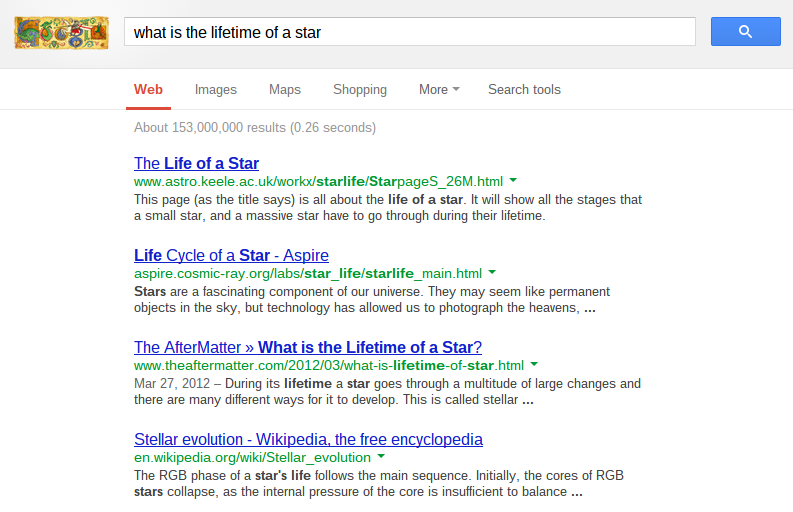
\includegraphics[width=0.9\textwidth]{google_search.png}
    \end{figure}
\end{frame}

\begin{frame}{Research}
    \begin{itemize}
        \item Not specifically physics, but essential part of the scientific method.
    \end{itemize}    
    \begin{figure}
        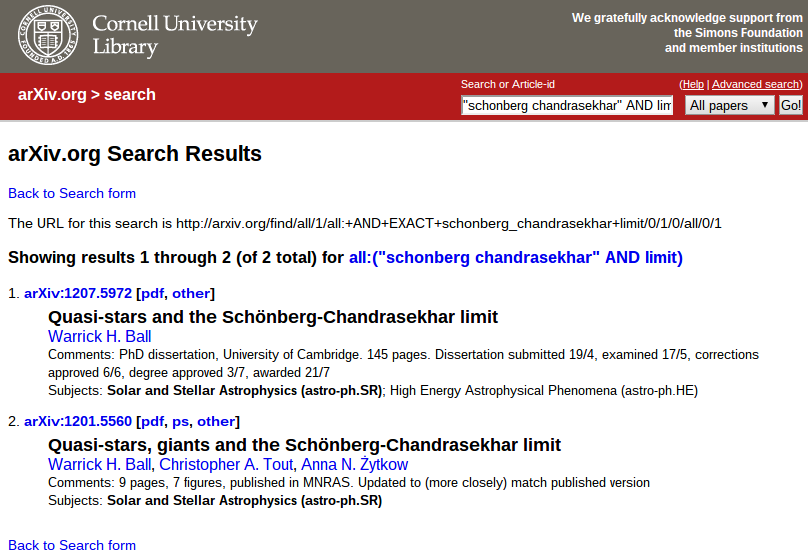
\includegraphics[width=0.9\textwidth]{arxiv_search.png}
    \end{figure}
\end{frame}

\begin{frame}{Interactivity}
    \begin{itemize}
        \item Brilliant tools available for teaching
        \begin{itemize}
            \item Videos - Youtube, Ted
            \item Animations - PhET
        \end{itemize}
    \end{itemize}
    \begin{figure}
        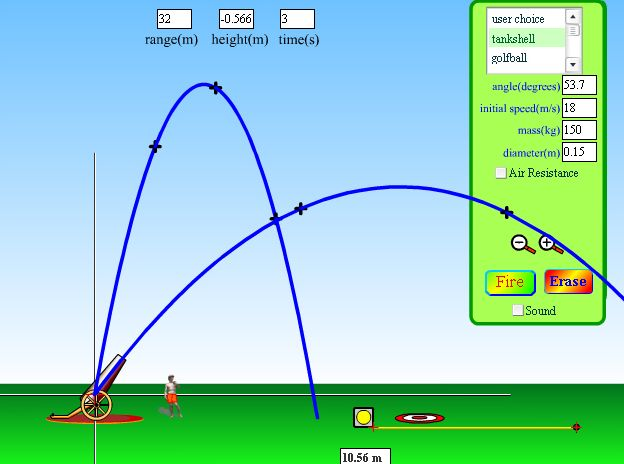
\includegraphics[height=4cm]{phet-1.jpg}
         ~
        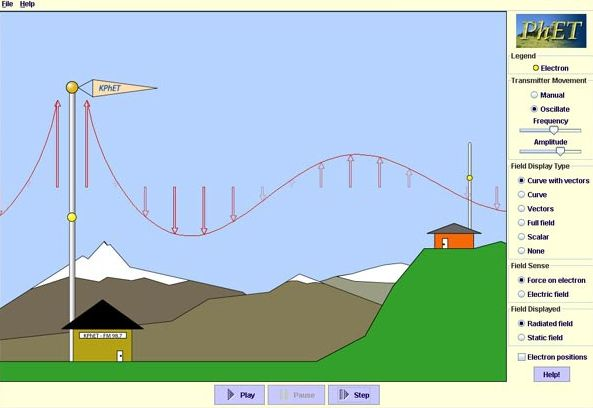
\includegraphics[height=4cm]{phet-2.jpg}
    \end{figure}
\end{frame}

\begin{frame}{Implementation}
    \begin{itemize}
        \item Computers and the internet are excellent resources
        \item Must be treated with caution to begin with
        \item Require education of teachers where needed \\~\\
        \pause
        \item Some decisions must be made
        \begin{itemize}
                \item is it always necessary and beneficial?
                \item how to introduce skills to students?
        \end{itemize}
        \\~\\
        \pause
        \item Why?
        \begin{itemize}
            \item Essential skills
            \item Advance beyond simple maths
        \end{itemize}
    \end{itemize}
\end{frame}

\end{document}
